\documentclass{article}

\usepackage{graphicx}
\usepackage[a4paper, margin=1in]{geometry}
\usepackage{amsmath}
\usepackage{IEEEtrantools}
\usepackage{karnaugh-map}

\graphicspath{{./assets/}}

\title{Assembly Lab 3}
\author{Aden Perry}
\date{\today}

\begin{document}
\maketitle

Captures show in order F, G, P, Q, and Result.

Input set 1 (P=9, Q=4):

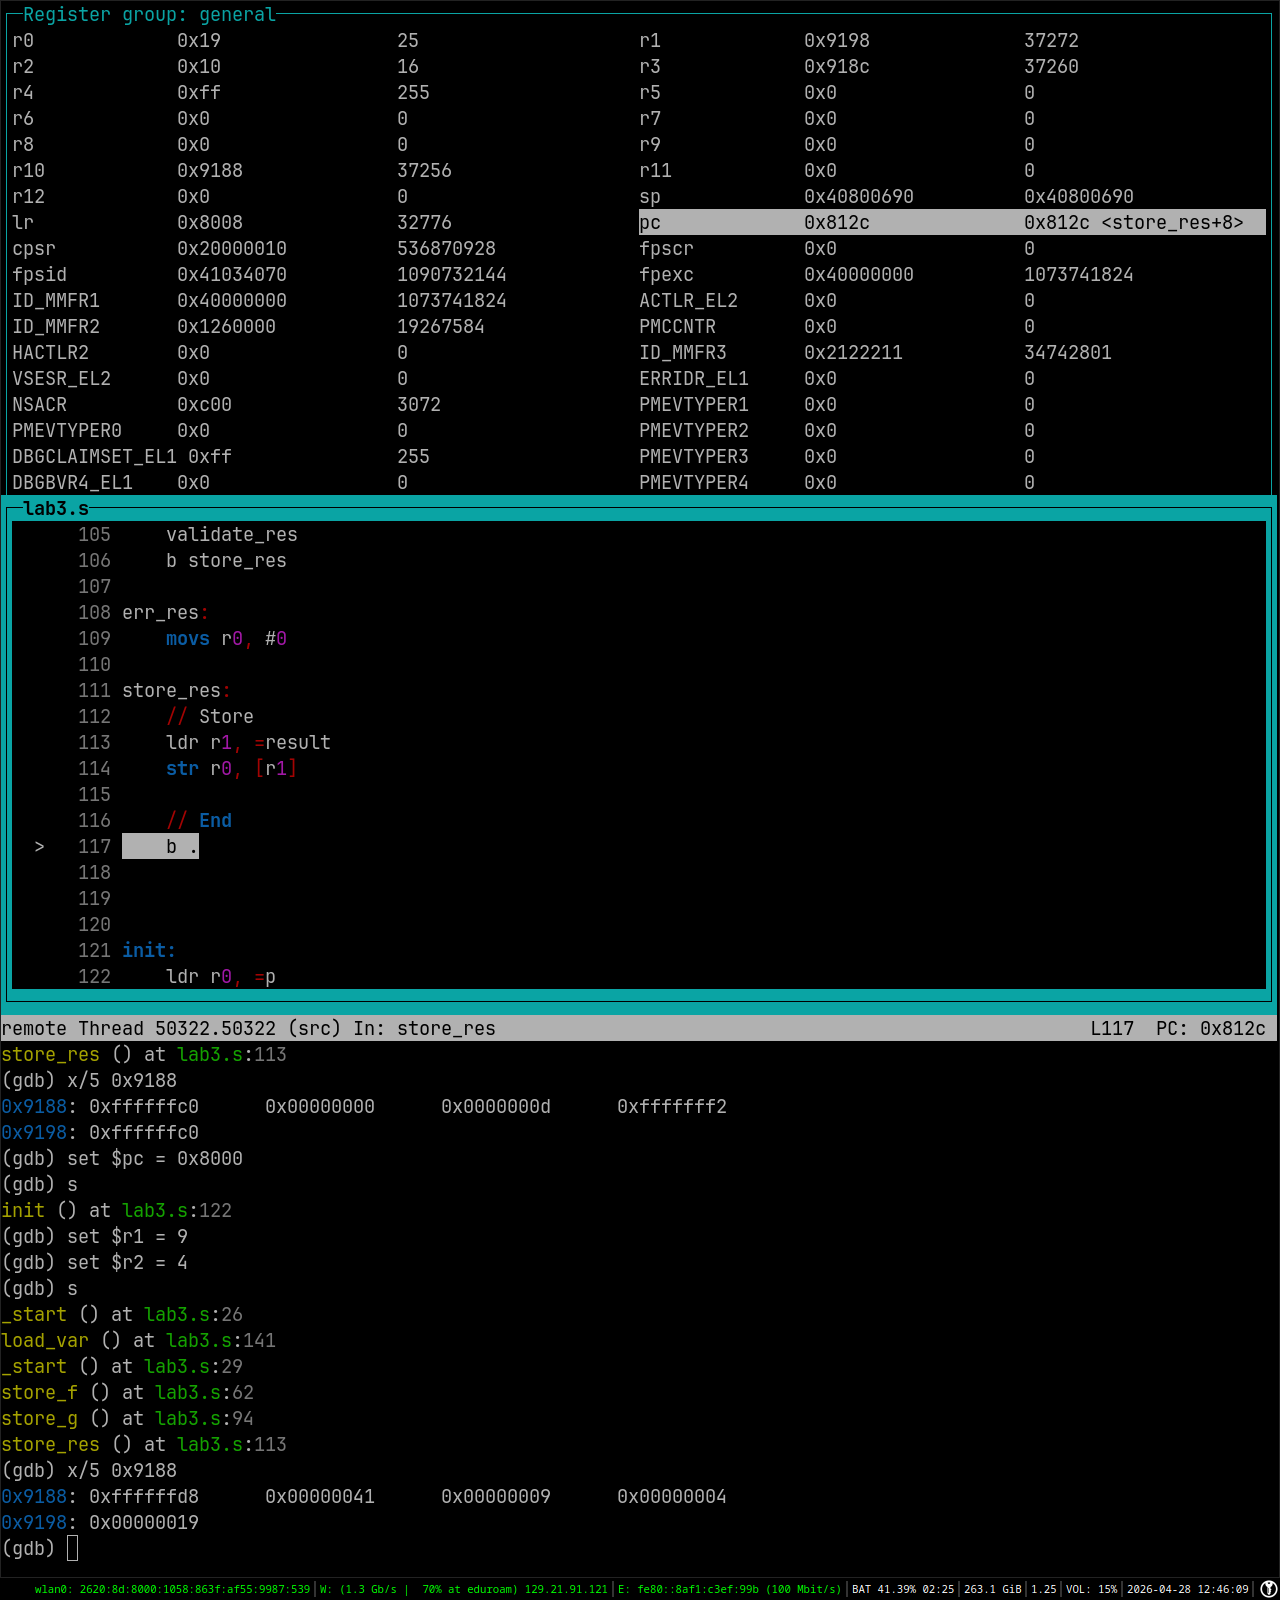
\includegraphics[width=0.8\textwidth]{val1.png}

Input set 2 (P=13, Q=-14):

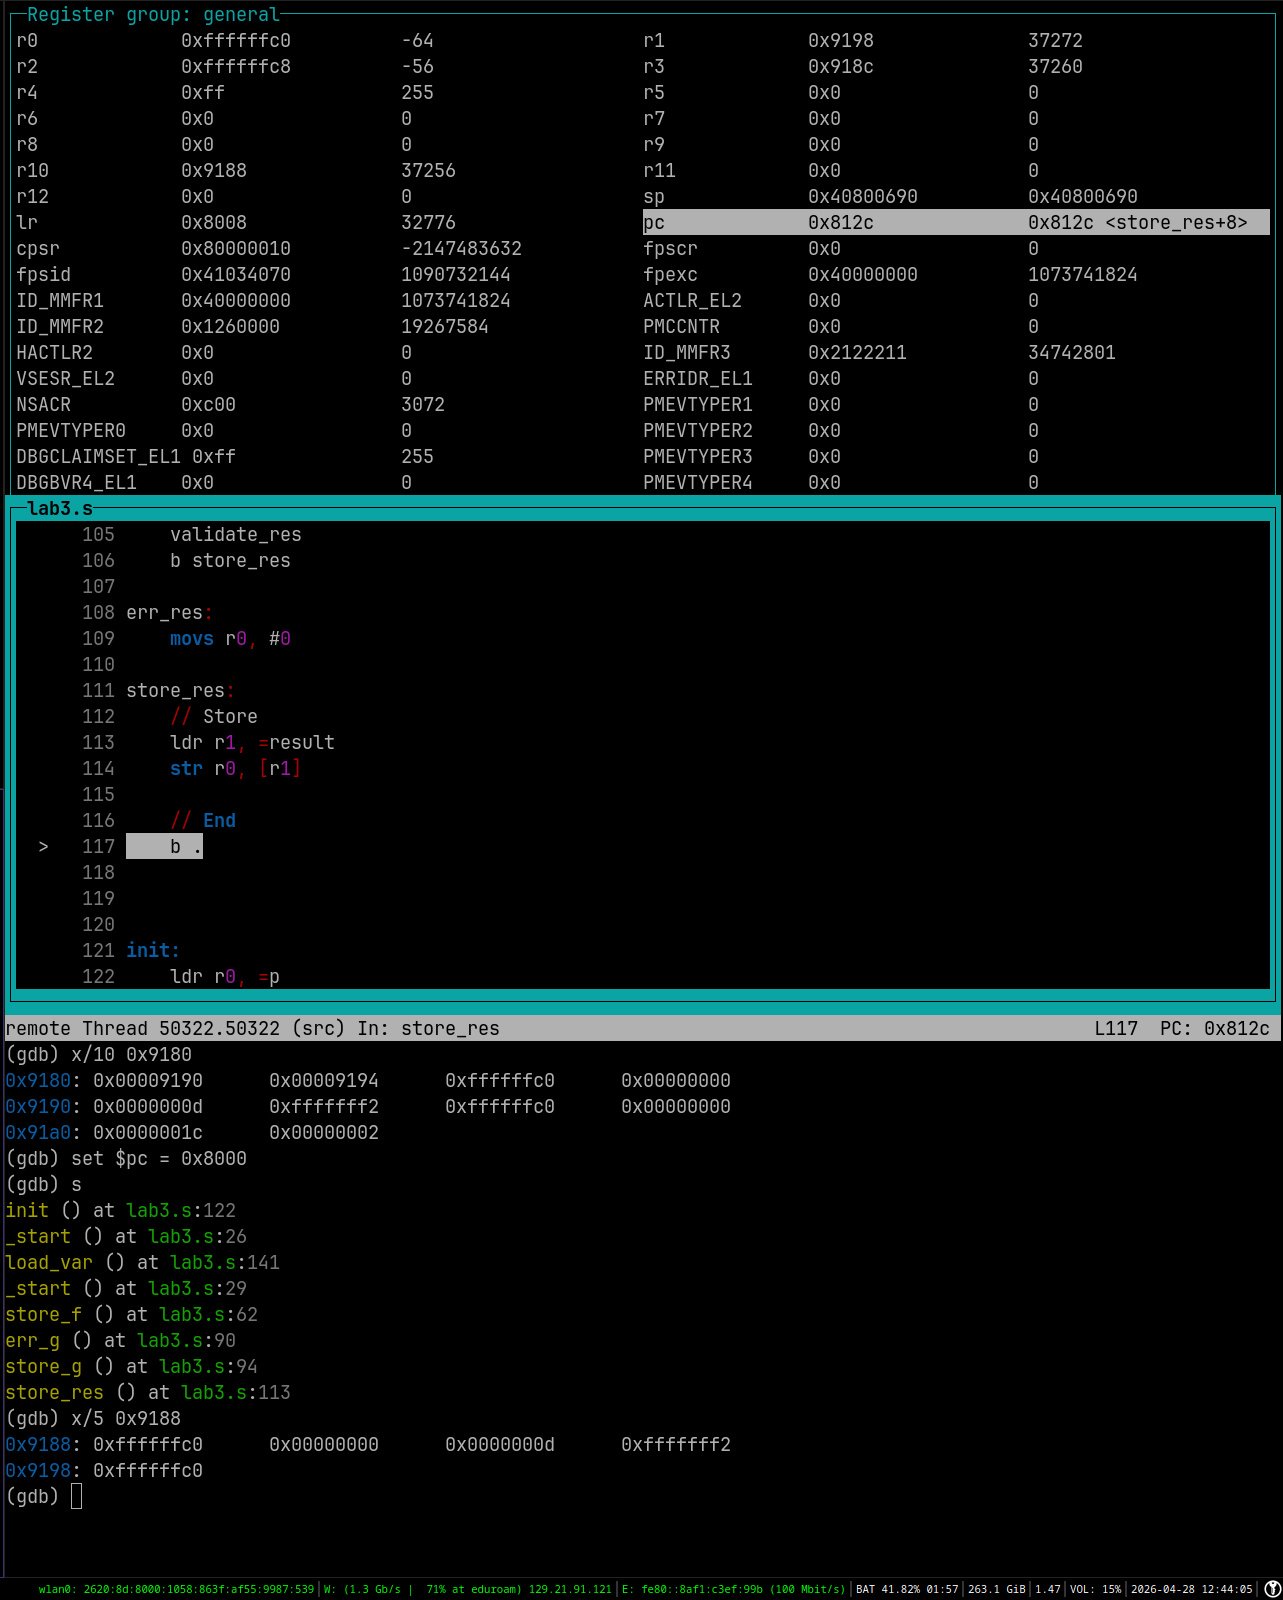
\includegraphics[width=0.8\textwidth]{val2.png}

Calculations:

\begin{align*}
	f = 3p + 2q - 75    \\
	3p = 3 \cdot 9 = 27 \\
	2q = 2 \cdot 4 = 8  \\
	27 + 8 = 35         \\
	35 - 75 = -40       \\
	g = 2p - 4q + 63    \\
	2p = 18             \\
	4q = 16             \\
	2p - 4q = 2         \\
	2 + 63 = 65         \\
	65 + -40 = 25
\end{align*}

In hex, f = 0xd8, g = 0x41, res = 0x19.

\begin{align*}
	f = 3p + 2q - 75                  \\
	3p = 3 \cdot 13 = 39              \\
	2q = 2 \cdot -14 = -28            \\
	39 + -28 = 11                     \\
	11 - 75 = -64                     \\
	g = 2p - 4q + 63                  \\
	2p = 26                           \\
	4q = -56                          \\
	2p - 4q = 82                      \\
	82 + 63 = 145 > 127 \Rightarrow 0 \\
	0 + -64 = -64
\end{align*}

In hex, f = 0xc0, g = 0x0, res = 0xc0.


Question:

Yes. Adding from right to left in the second input set would avoid overflow,
because it adds a large negative number before trying to handle two large
positive numbers.

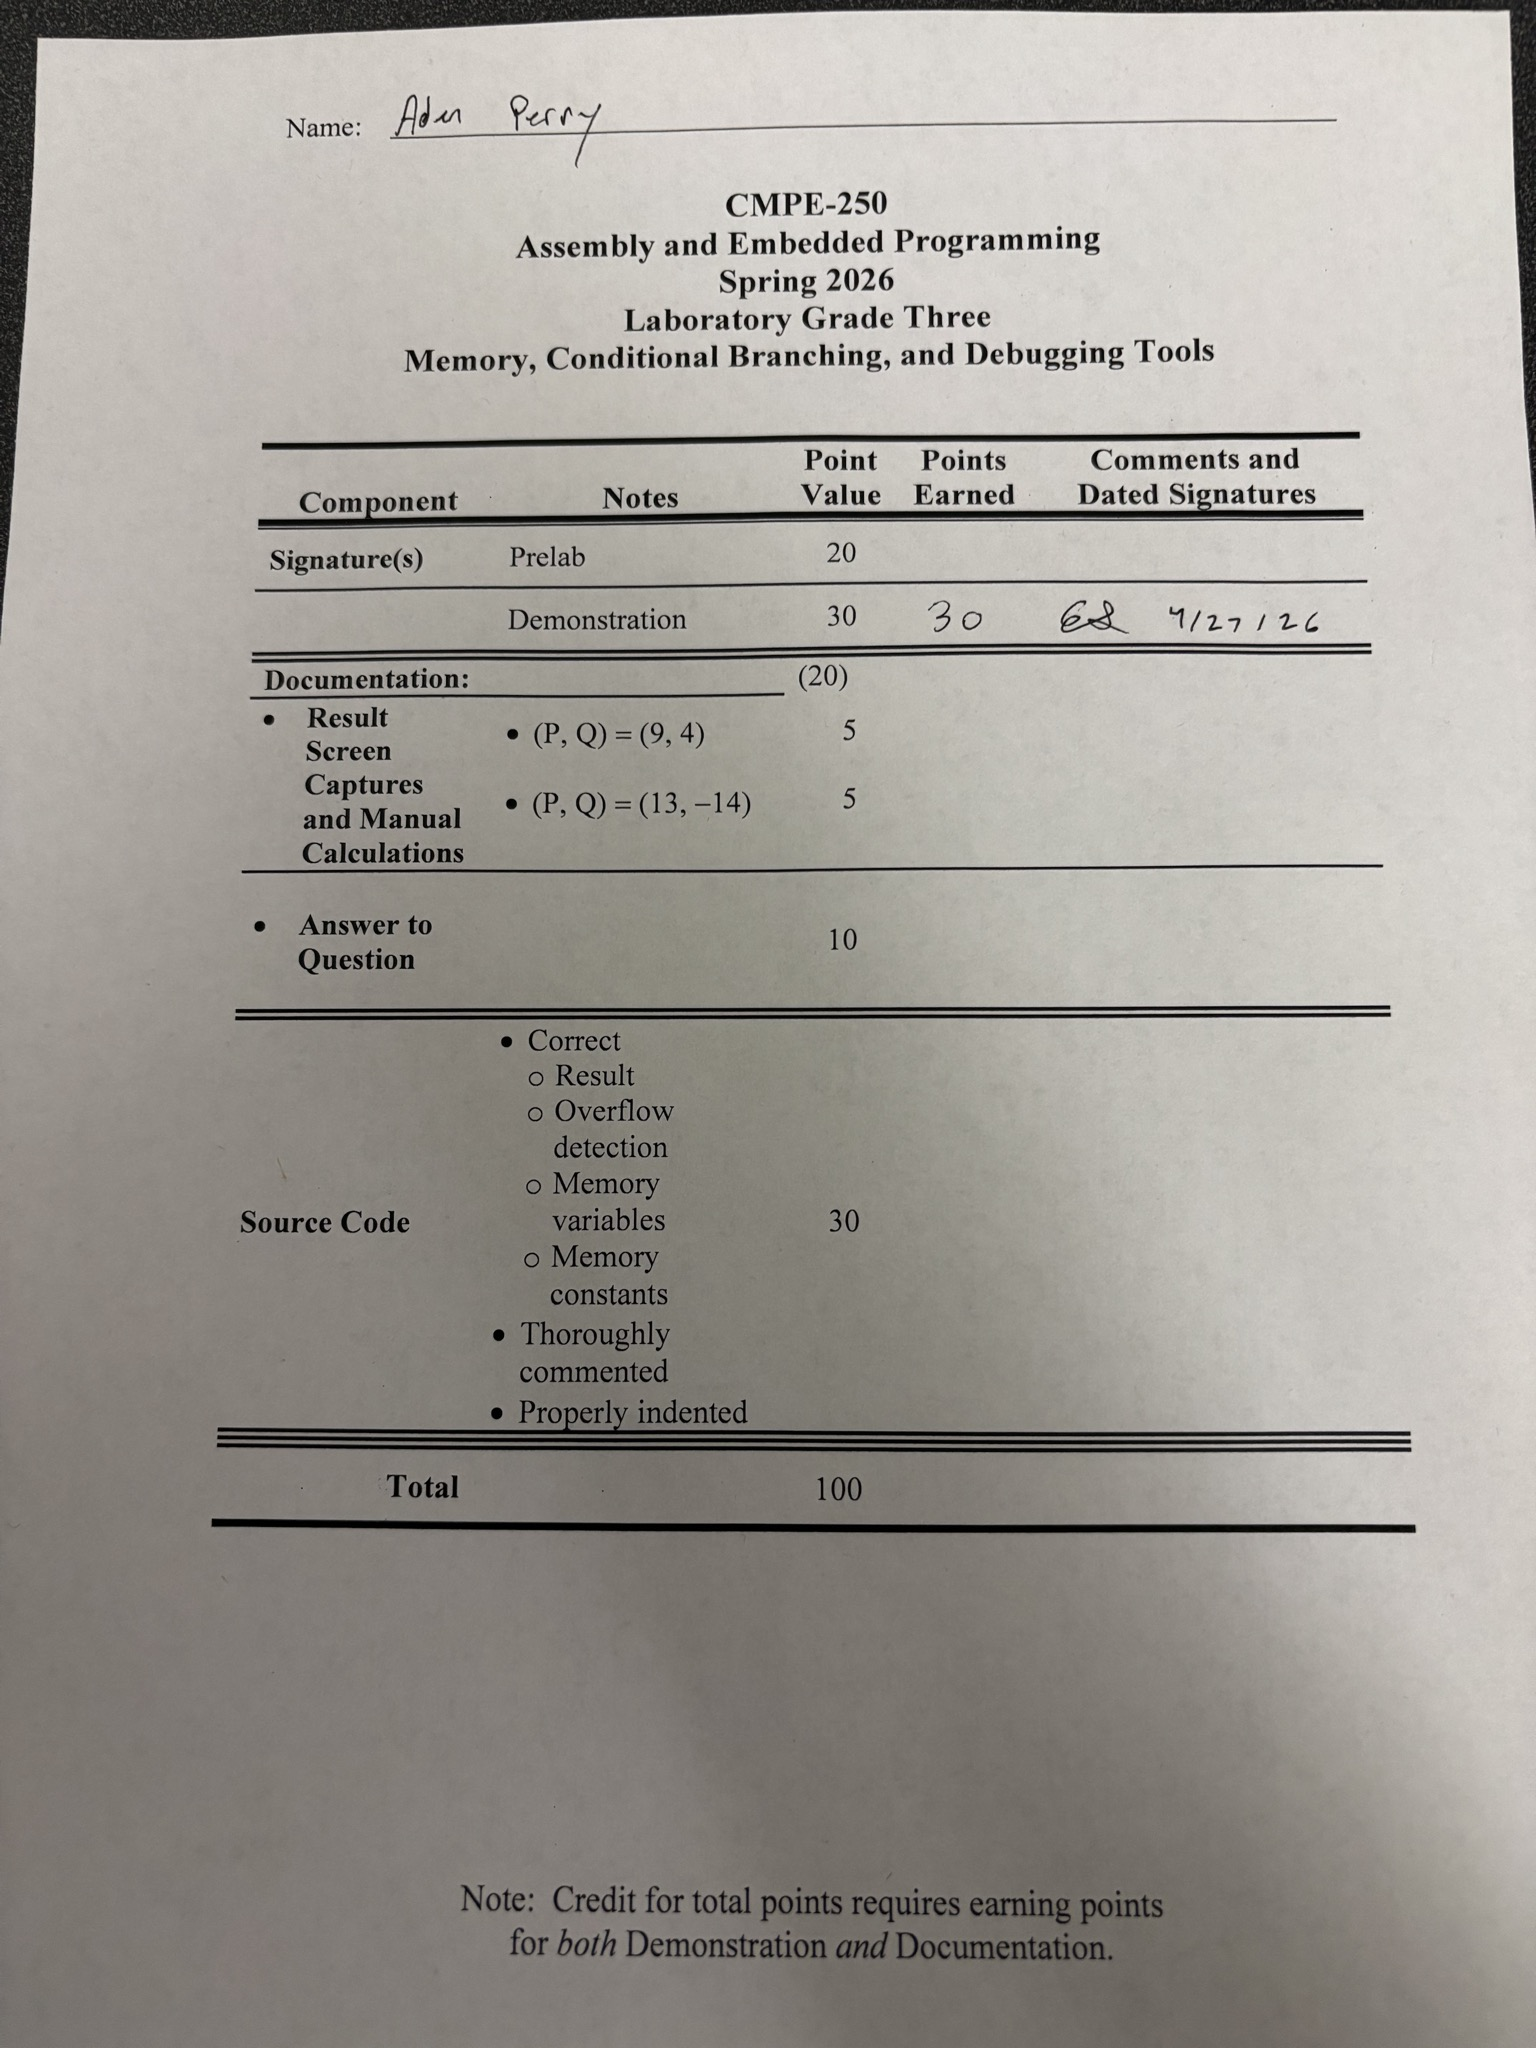
\includegraphics[width=\textwidth]{signoff.jpg}

\end{document}
